\documentclass[]{article}

% Packages

% Pseudocode
\usepackage{algpseudocode}
\usepackage{algorithm}

% Placing
\usepackage{float}
% Drawing
\usepackage{tikz}
% Memory maps
\usepackage{bytefield}
% Simple trees
\usepackage{qtree}
% Custom colors
\usepackage{xcolor}

% Plots
\usepackage{pgfplots}
\pgfplotsset{compat = newest}

% Dependencies
\usepackage{mymacros}


% Title
\title{Notes}
\author{Andrin Rehmann}

% Start
\begin{document}

\maketitle

\section{Introduction}


The N-Body technique has been used for decades to simulate the Universe so we can compare theory with observations. This technique uses ``particles'' or ``bodies'' to sample phase space, and as gravity operates over infinite distance it is necessary to consider all pair-wise interactions which makes a naive implementation $\mathcal{O}(n^2)$.
It is clear that this does not scale particularly well with large particle counts.

One common approach is to decompose the particles into a tree structure and multipole expansions of the particles in each tree cell to approximate the forces. This reduces the complexity of the algorithm to $\mathcal{O}(n\log{}n)$. More recently the Fast Multipole Method (FMM) has gained wider option primarily due to the extremely large sizes of modern simulations. This technique further reduces the complexity to $\mathcal{O}(n)$!

The computational effort required in modern N-Body simulations can thus be split into three categories:

\begin{itemize}
	\item \textbf{Load Balancing:} Distribute particles equally among nodes with regards to memory.
	\item \textbf{Tree Building:} Build tree on each node for accelerated force calculation and integration.
	\item \textbf{Force calculation and integration:} Calculate forces between particles and apply them.
\end{itemize}

Before the implementation of FMM into codes, and particularly before the era of modern accelerated computing (e.g., SIMD vectorization and GPU computing) the forces calculations dominated the computational cost. In more recent simulations, each category is about one third of the total calculation time\cite{2017ComAC...4....2P}. This makes the tree building and load balancing subjects to great performance gains, since GPU acceleration is usually not exploited. 

This project proposes to implement Tree Building with the GPU using CUDA to accelerate load balancing.


\section{Orthogonal Recursive Bisection (ORB)}


%https://de.overleaf.com/learn/latex/TikZ_package
%https://texample.net/tikz/examples/
The ORB Algorithm is used to partition a multi dimensional domain into subdomains based on spatial proximity. It does so by building an unbalanced binary tree. To explain the the algorithm we will refer to a left child of a node with index $i$ as $i*2$ and the right child respectively as $i*2 + 1$. The parent node can be determined with $\lfloor \frac{i}{2} \rfloor$. Finally we have $i = 1$ for the root node. Node that the actual code will not use the same system, but we will discuss this in a later section.

The advantage of subdividing the domain into smaller subdomains is two folds:

\begin{itemize}
	\item For simulation code and more specifically for the Fast Multipole Method these domains can be leveraged to greatly accelerate the simulation time. \TODO{expand}
	\item The workload can be equally distributed among nodes and processors in large computing systems.
\end{itemize} 

The general idea of the algorithm is to split a $k$ dimensional domain containing $N$ particles into $d$ subdomains using a recursive procedure. This can be repeated until the number of smallest subdomains is equal to the total count of processors or nodes. The final goal is an equal distribution of the workload and data, thus the subdomain sizes should be chosen such that the number of particles is equal among nodes / processors.

For a clearer terminology, we will refer to a node in the tree as a cell. The cell not only keeps track of its children, but also stores information about the domain it encompasses. In this tree the parent cell always encompasses the entire domains of its two child cells. Furthermore the domain of a child cell cannot exceed the boundaries of its parent domain. 

\subsection{Target Data}

\TODO{Write about properties of datasets}

\Q{Ask Doug}

\subsection{Computing Systems}

\TODO{Write about systems which can be used to test data and systems which are worth considering while estimating runtimes of this approach.}

\subsection{PKDGrav}

\TODO{Brief summary of PKDGrav and how this work can be used to improve PKDGrav}

\subsection{Memory and Workload Balancing}\label{sec:balancing}
During the simulation certain particles require more time steps, thus more computational effort, than others. We denote the workload per particle as the weighting function $w(p_i)$ where $p_i \in {p_1, p_2, ..., p_N}$.

Non equal weighting functions for different particles are due to higher accelerations and greater proximity to strong gravitational influences. This in turn requires a higher integrations accuracy to mitigate errors. When we try to balance the workload, this implies drawbacks in terms of memory balance. 

Let us consider a simple example to illustrate the point. Given the set of particles $A = {p_1, p_2, .., p_{2N/3}}$ and respectively $B = {p_{2N/3 + 1}, p_2, .., p_{N}}$. Let us now consider the that $\forall p \in A : w(p) = 1$ and $\forall p \in B : w(p) = 2$. If we assign all particles from set $A$ to process with rank 0 and the particles from B to rank 1. It is clear that $\sum_{p\in A}^{} w(p) = \sum_{p\in B}^{} w(p)$. Thus the two processors are balanced in terms of computing costs, but clearly they are not balanced in terms of memory size. In fact process with rank 0 has $2N/3$ elements and rank 1 has $N/3$ elements. Thus there will be processes there are memory slots which are not taken advantage of, which means we have a reduced total number of particles. As cosmological simulations profit from an increased number of particles, this also means that the quality of the simulation suffers when prioritizing workload balancing.


\subsection{ORB for power of twos}


Let us first make the assumption that $d$ is a power of two. In this case we can search for a cut such that 50\% of the particles are on the left side and likewise on the right side of the cut. The dimension of the cut is always the axis where the size of the domain is the largest. This ensures that we do not get thin shapes. \TODO{Insert smartness about FMM} This in turn is very beneficial for the FMM as it has a higher precision on more squarish shapes. After such a cut has been found, we can create two new subdomains and recursively apply the algorithm on both of them until we have reached the desired number of subdomains $d$. 
 
\vspace{5mm}

\def\x{8}
\def\y{8}
\def\s{5}

\def\spx{0.45}
\def\spya{0.5}
\def\spyb{0.6}
\begin{figure}[H]
\begin{center}
	\begin{tikzpicture}[scale=0.33]
		\pgfmathsetseed{2};
		\exdistr{\x}{\y}{\s};
		\draw (0,0) rectangle (\x, \y);
		\node[below] at (.5*\x,\y){$cell_1$};
	\end{tikzpicture}
	\qquad
	\begin{tikzpicture}[scale=0.33]
		\pgfmathsetseed{2};
		\exdistr{\x}{\y}{\s};
		\draw (0,0) rectangle (\x * \spx, \y);
		\node[below] at (.25*\x,\y){$cell_2$};
		
		\draw (\x  * \spx, 0) rectangle (\x, \y);
		\node[below] at (.75*\x,\y){$cell_3$};
		
		\vspace{2mm}
		
	\end{tikzpicture}
	\qquad
	\begin{tikzpicture}[scale=0.33]
		\pgfmathsetseed{2};
		\exdistr{\x}{\y}{\s};
		\draw (0,0) rectangle (\x * \spx, \y * \spya);
		\node[below] at (.25*\x,\y * \spya){$cell_4$};
		
		\draw (0,\y * \spya) rectangle (\x * \spx, \y);
		\node[below] at (.25*\x,\y){$cell_5$};
		
		\draw (\x * \spx,0) rectangle (\x, \y * \spyb);
		\node[below] at (.75*\x,\y * \spyb){$cell_6$};
		
		\draw (\x * \spx,\y * \spyb) rectangle (\x, \y);
		\node[below] at (.75*\x,\y){$cell_7$};
		
		\vspace{2mm}
	
\end{tikzpicture}
\end{center}
\caption{Building a tree of depth 3 using the ORB algorithm }
\label{fig:balorb}
\end{figure}

\vspace{5mm}

When each cell keeps track of its child cells, we have built a tree datastructure. For instance for our simple domain composition of depth 3 from Figure \ref{fig:balorb} we end up with structure as depicted in Figure \ref{fig:baltree} In this tree each cell represents a node, the root node is the cell which encompasses the entire space and particles and finally its leaves can be assigned to a processor / node. Note that the tree is not balanced, but each node has either two children or is a leaf. 

\begin{figure}[H]
\Tree[.cell_{1} [.cell_{2} [.cell_{4} ]
[.cell_{5} ]]
[.cell_{3} [.cell_{6} ]
[.cell_{7} ]]]
\caption{Tree datastructure of depth 3}
\label{fig:baltree}
\end{figure}

\subsection{ORB in the general case}

Let us now consider the general case where $d$ can be any integer number for a node with index $i$. In this case we define the desired number of particles on the left side of the cut as follows:

\begin{center}
	\begin{equation}
		l_{i} = \left \lceil \frac{ \lceil\frac{d_{i}}{2} \rceil }{d_{i}} \times N \right \rceil 
	\end{equation}
\end{center}

 Consequently the number of particles on the right side of the cut are: 
 
 \begin{center}
 	\begin{equation}
 		r_{i} = N - l_{i}
 	\end{equation}
 \end{center}
 
 The variable $d_{i}$ is defined in a recursive manner. We have $d_{i} = l_{\lfloor i/2 \rfloor}$ if $cell_i$ is a left child of its parent, otherwise we have $d_{i} = r_{\lfloor i/2 \rfloor}$.

\def\spya{0.5}
\def\spyb{0.5}
\begin{figure}[H]
	\begin{center}
		\begin{tikzpicture}[scale=0.33]
			\pgfmathsetseed{2};
			\exdistr{\x}{\y}{\s};
			\draw (0,0) rectangle (\x, \y);
			\node[below] at (.5*\x,\y){$cell_1$};
		\end{tikzpicture}
		\qquad
		\begin{tikzpicture}[scale=0.33]
			\pgfmathsetseed{2};
			\exdistr{\x}{\y}{\s};
			\draw (0,0) rectangle (\x * \spx, \y);
			\node[below] at (\spx * 0.5 * \x,\y){$cell_2$};
			
			\draw (\x  * \spx, 0) rectangle (\x, \y);
			\node[below] at (0.63 *\x,\y){$cell_3$};
			
			\vspace{2mm}
			
		\end{tikzpicture}
		\qquad
		\begin{tikzpicture}[scale=0.33]
			\pgfmathsetseed{2};
			\exdistr{\x}{\y}{\s};
			\draw (0,0) rectangle (\x * \spx, \y);
			\node[below] at (\spx * 0.5 * \x,\y){$cell_4$};
			
			\draw (0,0) rectangle (\spx * \x, \y * \spyb);
			\node[below] at (.25*\x,\y * \spyb){$cell_5$};
			
			\draw (\x * \spx,0) rectangle (\x, \y);
			\node[below] at (.75*\x,\y){$cell_3$};
			
			\vspace{2mm}
			
		\end{tikzpicture}
	\end{center}
	\caption{Building a tree of depth 3 using the ORB algorithm }
\end{figure}

\begin{figure}[H]
	\Tree[.cell_1 [.cell_2 [.cell_4 ] [.cell_5 ] ]
	[.cell_3 ]]
	\caption{Tree datastructure of depth 3}
\end{figure}


\subsection{Median Finding Algorithms}

Finding the median of a large particle array is an essential step for ORB. We will thus explore different algorithms alongside their advantages and disadvantages for our specific use case.
Note that there exists approximation algorithms for example the median of medians algorithms. But the correctness guarantee of the median lying between 30\% and 70\% is not good enough in our case. If we were to implement such an approximation algorithms we would run into similar issues as described in \ref{sec:balancing}. But in this case the unequal memory balancing do not have the advantage of equal workload balancing, which in turn will worsen the performance and the maximum number of workable particles. Thus we will only consider approximation algorithms, if their approximation to the ideal values are very exact and can be determined.

\subsubsection{Binary Search}
The simplest algorithm is the binary search algorithm. It always cuts the domain in half along a given axis. Next it counts the number of particles on the left side of the cut, in case the particles are less than half of all the particles, it clear that the cut was too far to the left, and the new right boundary of the domain is the cut. In case the particles are more than half, we set the the left boundary as the cut. This is repeated until we either reach an exact split, a cut-off value or reach the precision limit of the data.


\begin{algorithm}[H]
	\caption{Find cut algorithm}\label{algo:cut}
	\begin{algorithmic}[1]
		\Procedure{cut}{$left, right, axis ,particles$}
		\State $nLeft = 0$
		\State $split = (right - left) / 2 + left $ \Comment{Initial guess}
		\While{$abs(nLeft - particles.length/2) > 1 $}
		\State $split = (right - left) / 2 + left $
		\State $nLeft\gets sum(particles[:,axis] < split)$
		\If{$nLeft <= particles.len / 2$}
		\State $left = split$
		\Else 
		\State $right = split$
		\EndIf
		\EndWhile\label{euclidendwhile}
		\State \Return $split$
		\EndProcedure
	\end{algorithmic}
\end{algorithm}

We analyse the runtime of the cut algorithm as follows: Inside the loop we need to count the number of particles on the left side of the cut. Since the particles are not ordered, we need to sweep over all particles which leaves us with a runtime of $O(N)$. Furthermore we need to estimate the number of times the while loop is repeated. We denote the precision of the cut as $p$. This means the cut operation is stored with $p$ bits. 
Let us consider the case where we search for the split on an integer domain of the size $2^{32}$ which equates a 32 bit precision integer number. With each iteration we cut in half the integer domain. Thus after the first iteration the domain size is $2^{31}$. It is therefore where easy to verify that a maximum of 32 repetitions can be performed before our domain reaches a size of $2^0$. In this case the cut cannot be improved as it has already reached the maximum precision. We conclude a worst case performance of $O(N \times 32)$. 

The average case is harder to estimate and it also depends on the number of particles. Let us assume a uniform random distribution of particles. In this case the average distance between two particles is $\frac{2^{p}}{N}$. \TODO{Extend}

\subsubsection{Binary Search with improved guessing}

As we can see in \ref{algo:cut}, the initial guess of the cut is simply the center of the domain. But if we consider non uniform distributions, this initial guess can possibly rather bad. Let us consider the following example:

\begin{figure}[H]
	\begin{center}
		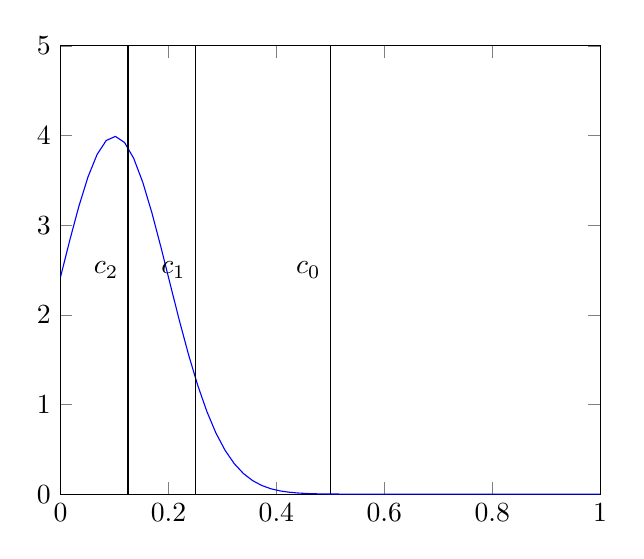
\begin{tikzpicture}
			\def\mean{0.1}
			\def\sigma{0.1}
			\def\pi{3.14159265359}
			\begin{axis}[xmin = 0, xmax = 1, ymin=0, ymax=5, samples=60]
				\addplot[domain = 0:1,blue] {1 / (\sigma * sqrt(2 * \pi)) * exp(-0.5 * ((x - \mean) / \sigma)^2) };
				\draw (axis cs:0.5,0) -- node[left]{$c_0$} (axis cs:0.5,5);
				\draw (axis cs:0.25,0) -- node[left]{$c_1$} (axis cs:0.25,5);
				\draw (axis cs:0.125,0) -- node[left]{$c_2$} (axis cs:0.125,5);
			\end{axis}
		\end{tikzpicture}
	\end{center}
	\caption{3 iterations of binary search with naive initial guess}\label{euclid}
\end{figure}

The underlying distribution is a normal distribution. \TODO{Add reference to section about data}. We can see that the algorithm will have to sweep 3 times over the entire array to get into the region of the actual median. One suggestion for improvement is to use an approximated median as a guess for the first split. We can sample 100 particles and find their median in constant time. Then we will run the binary cut algorithm using the approximated median as an initial guess. This can reduce the runtime by a few iterations, however we cannot make any assessment about the runtime, as this improvement will make the algorithm even slower on some distributions. Let us for example consider the uniform distribution, in this case the addition is pure overhead as the center is already the most accurate initial guess.


\subsubsection{Binary search with early stopping}


\subsubsection{Histogramming}




\subsection{Reshuffling Algorithm}

\begin{algorithm}[H]
	\caption{Reshuffle algorithm}\label{euclid}
	\begin{algorithmic}[1]
		\Procedure{reshuffle}{$cut, axis ,particles$}
		\State $i = 0$
		
		\For{j in {0,..,particles.len() - 1}}
		\If{$particles[js,axis] < split$}
		\State $i = i + 1$
		\State $particles.swap(i,j)$
		\EndIf
		\EndFor
		
		\State $particles.swap(i,particles.len() - 1)$
		\State \Return $i$
		\EndProcedure
	\end{algorithmic}
\end{algorithm}

The reshuffle algorithm has a clearly observable runtime of $O(N)$ since we iterate over all particles once. Since we need to touch each element at least once to reshuffle the entire array there is no better algorithm than this.

\subsection{ORB Main routine}

\begin{algorithm}[H]
	\caption{The ORB main routine}\label{euclid}
	\begin{algorithmic}[1]
		\Procedure{orb}{$cornerA, cornerB ,particles, np$}
		\State $size = cornerB - cornerA$
		\State $axis = maxIndex(size.x, size.y, size.z)$ \Comment{Get index of max size}
		
		\State $left = cornerA[axis]$
		\State $right = cornerB[axis]$
		\newline
		\State $cut = cut(left, right, axis, particles)$
		\State $mid = reshuffle(split, axis, particles)$
		\newline
		
		\TODO{Finish this}
		\State \Call {orb}{cornerA, cornerB}
		\EndProcedure
	\end{algorithmic}
\end{algorithm}


\vspace{5mm}


\section{Theoretical analysis of ORB speedup by GPU acceleration}

In order to have a broad idea what speedup we can expect by implementing a GPU version, we first need to understand which parts of the code are suited to be done on the GPU. The GPU profits from a highly parallelized architecture, this means that it performs exceptionally when vectorization can be applied to large set of values. But the GPU has another strength over the CPU, which may be lesser known. The memory bandwidth between the GPU and its memory is much greater than the memory bandwidth between the CPU and GPU. Since the time used for calculations is a lot smaller due the algorithm only requiring few and simple operations and is negligible in comparison to memory loading times, we omit speed-ups which are introduced by parallelizing calculations and instead focus on the memory access times. Thus for the section of theoretical analysis we assume that the waiting function is always $w(p) = 0$.

To analyse the runtime for the CPU we are using Equation \ref{eq:cpu}. For the analysis we make following assumptions:

\begin{itemize}
	\item
	One particle consists of an X, Y and Z coordinate, each stored as a $p$ = 32 bit = 8bytes precision number. Thus the combined  XYZ coordinates require $4\times3 = 12$ bytes of storage.
	
	\item 
	All particles are assumed to be stored in the CPU memory initially.
	
	\item
	We perform the analysis on one billion particles. This translates to $10^9 \times  12 bytes = 12 GB$.
	
\end{itemize}

\TODO{Find tflops}

% Compare flops with speed of memory
% Add small experiment
% Memory Bandwidth Cliff
Let us assume a CPU with a clock speed of $cps$ per second. 

\subsection{Runtime estimations on a single node}

\TODO{Add introduction}

\subsubsection{Naive implementation}

\begin{center}
	\begin{equation}
			p \times \frac{ s }{B_{CPU}} = t
			\label{eq:cpu}
	\end{equation}
\end{center}

\vspace{5mm}


The Equation \ref{eq:gpu} for the GPU is similar, the only difference being that we use the GPU memory bandwidth $B_{GPU}$ instead of the CPU bandwidth. Furthermore we have to consider the time it takes to send the data from the CPU to the GPU. This adds the terms size divided by CPU to GPU memory bandwidth denoted as $I$. Finally we also need to load the data from the CPU memory to the CPU before we are able to send it. 

\begin{center}
	\begin{equation}
		p \times \frac{s}{B_{GPU}} + \frac{s}{I}  + \frac{s}{B_{CPU}}= t
		\label{eq:gpu}
	\end{equation}
\end{center}

\vspace{5mm}


\subsubsection{GPU tree building}

Let us now consider an alternative way of computing binary cuts. We will build part of the tree on the GPU itself. This will allow us to reduce the very costly overheads imposed by transferring data from the CPU to the GPU. The maximum number of cuts we can perform is $p \times 3$. After p cuts we have $2^{p \times 3}$ leaf cells, and have reached the precision. Note that in this case we also need to send back the information about the built tree from the GPU to the CPU. 

\TODO{Too strong of a simplification}
\begin{center}
	\begin{equation}
		d \times p \times \frac{s}{B_{CPU}} = t
		\label{eq:cputree}
	\end{equation}
\end{center}

\begin{center}
	\begin{equation}
		d \times p \times \frac{s}{B_{GPU}} + 2 \times \frac{s}{I} = t
		\label{eq:gputree}
	\end{equation}
\end{center}


\subsubsection{Batch loading}

Finally we can also try to mitigate the overheads introduced by CPU to GPU communication by sending small batches, such that the GPU can already start processing the data, before the data transfer was completed. Lets denote the number of batches by $b$. For the sake of simplicity we only make a single cut and thus can reuse Equation \ref{eq:cpu} for the CPU version. For the GPU we now omit the term for memory access from the GPU. Because we can already start processing data in parallel when the first batch arrived and $B_{GPU} > I$ holds for every modern hardware. Thus the only overhead we still get is $\frac{s \div b}{B_{GPU}}$ for the very last batch, but as we can just increase b in relation to N, this becomes negligible. Note that this only counts for the very first iteration, thus the only difference we have is the constant of 31 and not 32. 

\begin{center}
	\begin{equation}
		(d-1) \times p \times \frac{s}{B_{GPU}} + 2 \times \frac{s}{I} = t
		\label{eq:gpubatch}
	\end{equation}
\end{center}

Due to possible overhead and no real improvement over the naive GPU version, we will omit the analysis using this method.

\subsubsection{Data compression}

Since for most computer the Interconnect bandwidth is greatly smaller than the Memory Bandwidth, we could potentially also think about compressing the particle data. This would increase computational costs, but would allow us to store a higher amount of particles and reduce the cost which comes from loading the particles from memory as well as sending the data over the Interconnect.

\begin{itemize}
	\item Why do we even use floats in the first place? wouldn't integers suit better since precision is uniformly equal?
	\item Reduce transfered number of bits, sacrifice precision?
\end{itemize}

\TODO{Add plots?}
\subsection{Datapoints of supercomputers}

We will compare the performance with the datapoints of Piz Daint, Summit and Alps which is a part of Eiger. We choose Piz Daint because we have the possibility to test the Code on its systems. We choose Eiger because we can also access its systems and it will give us a good reference values, due to it being a non hybrid supercomputer, meaning the nodes to not have GPU. Finally we analyze its performance on Summit, as its at the time of writing this thesis, one of the most capable supercomputers in the world.

\small
\begin{figure}[H]
	\begin{center}
		\begin{tabular}{ c c c c }
			& Piz Daint \cite{piz_daint} & Summit & Alps (Eiger) \\ 
			\hline
			Number of Nodes & 5704 & 4608 & 1024\\
			CPU Mem. Cap. & 64 GB & 256 GB $\times$ 2  \\   
			CPU Model & Intel E5-2690 v3 & IBM POWER9 $\times$ 2 & AMD EPYC 7742 \\
			CPU Mem. Bandw.  & 68 GB/s & 170 GB/s & 204.8 GB/s x 2	\\
			GPU Model & NVIDIA P100 & NVIDIA V100s  $\times$ 6 & None \\
			GPU Mem. Cap. & 16 GB & 16 GB $\times$ 6 & -\\
			GPU Mem. Bandw. & 732 GB/s & 900 GB/s & -\\
			Interconnect Bandw. & 32 GB/s & 50 GB/s & -\\
		\end{tabular}
	\end{center}
\caption{Datapoints of Supercomputers}
\label{fig:datapoints}
\end{figure}

We can now plug-in the values we obtained from different supercomputers in our equations.  We will assume a precision $p = 32$ bits which is sensible in the case of astrophysical simulations. \TODO{Add reference}.

\normalfont
\subsection{Piz Daint} 

Let us plugin the values from Figure \ref{fig:datapoints} into the corresponding formulas \ref{eq:cpu}, \ref{eq:gpu}, \ref{eq:cputree} and \ref{eq:gputree}.

\subsubsection{Naive implementation}
The naive implementation yields the following speeds for the naive CPU  implementation:

\begin{center}
	\begin{equation}
		32 \times \frac{ 12 GB }{68 GB/s} = 5.65s
	\end{equation}
\end{center}


And the corresponding GPU implementation:
\begin{center}
	\begin{equation}
		32 \times \frac{12 GB}{732 GB/s} + \frac{12 GB}{32 GB/s}  + \frac{12 GB}{68 GB/s} = 1.08s
	\end{equation}
\end{center}


%\begin{tikzpicture}
%	\begin{axis}[xmin = -1, xmax = 13, ymin=-1, ymax=6]
%		\addplot[domain = 0:12,blue] {(32 * x / 68) / (32 * x / 732 + x /32 + x/68) };
%	\end{axis}
%\end{tikzpicture}

This yields in a speed-up of:
\begin{center}
	\begin{equation}
		\frac{5.65s}{1.08} = 5.25
	\end{equation}
\end{center}


\subsubsection{GPU Tree Building}

\begin{center}
	\begin{equation}
		32 \times 32 \times \frac{ 12 GB }{68 GB/s} = 180s
	\end{equation}
\end{center}

And the corresponding GPU implementation:
\begin{center}
	\begin{equation}
		32 \times 32 \times \frac{12 GB}{732 GB/s} + 2 \times \frac{12 GB}{32 GB/s}  + \frac{12 GB}{68 GB/s} = 17.71s
	\end{equation}
\end{center}

This yields in a speed-up of:
\begin{center}
	\begin{equation}
		\frac{180s}{17.71} = 10.2
	\end{equation}
\end{center}

\vspace{5mm}


\subsection{Summit}

Let us plugin the values from Figure \ref{fig:datapoints} into the corresponding formulas \ref{eq:cpu}, \ref{eq:gpu}, \ref{eq:cputree} and \ref{eq:gputree}.

\subsubsection{Naive implementation}
The naive implementation yields the following speeds for the naive CPU  implementation:

\begin{center}
	\begin{equation}
		32 \times \frac{ 12 GB }{170 GB/s \times 2} = 2.56s
	\end{equation}
\end{center}

And the corresponding GPU implementation:
\begin{center}
	\begin{equation}
		32 \times \frac{12 GB}{900 GB/s \times 6} + \frac{12 GB}{50 GB/s \ times 6}  + \frac{12 GB}{170 GB/s \ times 2} = 0.74s
	\end{equation}
\end{center}

This yields in a speed-up of:
\begin{center}
	\begin{equation}
		\frac{2.56s}{0.74s} = 3.06
	\end{equation}
\end{center}


\subsubsection{GPU Tree Building}

\begin{center}
	\begin{equation}
		32 \times 32 \times \frac{ 12 GB }{170 GB/s} = 70.28s
	\end{equation}
\end{center}

And the corresponding GPU implementation:
\begin{center}
	\begin{equation}
		32 \times 32 \times \frac{12 GB}{900 GB/s} + 2 \times \frac{12 GB}{50 GB/s}  + \frac{12 GB}{170 GB/s} = 14.2s
	\end{equation}
\end{center}

This yields in a speed-up of:
\begin{center}
	\begin{equation}
		\frac{70.28s}{14.2s} = 4.95
	\end{equation}
\end{center}


\vspace{5mm}


\subsection{Eiger}

\begin{center}
	\begin{equation}
		32 \times 32 \times \frac{ 12 GB }{204.8 GB/s} = 60s
	\end{equation}
\end{center}

\subsection{Conclusion}

We conclude that the GPU version with GPU Tree building enabled yields the best speedup and also performs a lot better than the CPU version. Also we can observe that the speedup is bounded by $\frac{B_{GPU}}{B_{CPU}}$/ \TODO{Add reasoning}

\section{Implementation}

\subsection{Data-structure}

\subsubsection{Tree}

The data-structure which stores the entire three needs to have following properties:

\begin{itemize}
	\item store domain information and provide access to left and right child cells
	\item Allow highly unbalanced trees
\end{itemize}

The most naive approach is to use a struct for each cell which stores information about the domain and keeps a pointer to the left and right cell. However since we in high performance systems, synchronizing pointers can be a bit of hassle, furthermore PKDGrav implements distributed arrays. Thus we can store all domain information in an array and simply keep track of the indices of its child cells. This can even be reduced further, since the right child cell is being created by the same process as the left child was. Thus we can assign the information about the right child in the positions left + 1 and only keep track of the index of the left child.

The minimal amount of data we need to store for each cell is its exact boundaries, the begin and end index in the particles array, and finally a index of the left child. If we sketch out two cells as a memory layout it looks as follows:
\begin{figure}[H]
	\begin{center}
		\begin{bytefield}{24}
			\begin{rightwordgroup}{cell 0}
				\memsection{0}{32}{2}{lower x}\\
				\memsection{32}{64}{2}{lower y}\\
				\memsection{64}{96}{2}{lower z}\\
				\memsection{96}{128}{2}{upper x}\\
				\memsection{128}{160}{2}{upper y}\\
				\memsection{160}{192}{2}{upper z}\\
				\memsection{192}{224}{2}{begin}\\
				\memsection{224}{256}{2}{end}\\
				\memsection{256}{288}{2}{left child}\\
			\end{rightwordgroup}\\
			\begin{rightwordgroup}{cell 1}
				\memsection{288}{320}{2}{lower x}\\
				\memsection{320}{352}{2}{lower y}\\
				\memsection{352}{384}{2}{lower z}\\
				\memsection{384}{416}{2}{upper x}\\
				\memsection{416}{448}{2}{upper y}\\
				\memsection{448}{480}{2}{upper z}\\
				\memsection{480}{512}{2}{begin}\\
				\memsection{512}{544}{2}{end}\\
				\memsection{544}{576}{2}{left child}\\
			\end{rightwordgroup}\\
			
		\end{bytefield}
	\end{center}
\end{figure}

Note that in theory we could only store the split position and axis for each particle, which would only require 32 bits for the positions and 2 bits (for 3D) for the axis. However the exact domain information can then only be achieved by traversing the three starting from the root. We can however make use of this data-structure when the communication overhead is greater than the costs of reconstructing the datastrucutre. Thus this storage version can be thought of as a lossless data compression of the tree.
\subsubsection{Particles}

The particles need to be stored in an array. We can implement the array using c style arrays, std::array or even an std::vector. The disadvantage of std::array and std::vector is their speed. On the other c-style arrays are limited in terms of multi dimensional indexing and boundary checking. Thus we make use of the library blitz++ which combines the speed of C-style arrays with the functionality of the std::vector. Furthermore blitz++ uses the same memory layout we would expect from a C-style array which looks as follows:

\begin{figure}[H]
	\begin{center}
		\begin{bytefield}{24}
			\begin{rightwordgroup}{particle 0}
				\memsection{0}{32}{4}{x}\\
				\memsection{32}{64}{4}{y}\\
				\memsection{64}{96}{4}{z}\\
			\end{rightwordgroup}\\
			\begin{rightwordgroup}{particle 1}
				\memsection{96}{128}{4}{x}\\
				\memsection{128}{160}{4}{y}\\
				\memsection{160}{192}{4}{z}\\
			\end{rightwordgroup}\\
		
		\end{bytefield}
	\end{center}
\end{figure}

\TODO{Data compression notice here?}


\subsection{Parallel Version Using Processes}

To parallelize the ORB algorithms, we first need to think about which parts of the algorithm can be parallelized and yield in a performance improvement. The most obvious choice for parallelization is the counting part from the binary cut algorithm. In this case the main thread (rank 0) will send a cut position and each processor counts how many particles there are on the left of this cut positions. It does so in a designated range of the entire particle array, which is unique to each rank.

\subsubsection{Local Reshuffling}

\begin{figure}[H]
	\begin{center}
		\begin{tikzpicture}
				
			\timeline{6}{16}{3}
			
			
			\parallelloop{-2}{15.5}{8}{0.5}{loop till all cells found};
		
			\parallelloop{-1}{11.5}{7}{3.5}{loop till cut found};
			
			\communication{Broadcast cells}{0}{7}{15};
						
			\process{local\\ reshuffle}{0}{14};
			\process{local\\ reshuffle}{2}{14};
			\process{local\\ reshuffle}{4}{14};
			\process{local\\ reshuffle}{6}{14};
			
			\process{compute\\ cut}{0}{11};
			
			 
			\communication{Broadcast cut from operative}{0}{7}{8};
			
			\process{local \\ count}{0}{7};
			\process{local \\ count}{2}{7};
			\process{local \\ count}{4}{7};
			\process{local \\ count}{6}{7};
	
			
			\communication{Reduce count to operative}{0}{7}{4};
			
			\process{generate\\ new \\ cells}{0}{3};

		\end{tikzpicture}
	\end{center}
\caption{Parallelized ORB for np = 4 and local reshuffling}
\label{fig:orb_parallel}
\end{figure}

\subsubsection{Global Reshuffling}

Another strategy we can use, as soon as we have created two domains, rank 0 can process one domain and rank 1 can process the other domain. This has the advantage that not only the counting part, but also the costly reshuffling part of the ORB algorithm can be parallelized. Furthermore the amount of data which needs to be communicated between the different threads is smaller. This is due to the fact that as soon as we found our first cut, only half the array of particles 


\begin{figure}[H]
	\begin{center}
		\begin{tikzpicture}
			
			\timeline{6}{8}{3}

			\communication{Compute cut}{0}{7}{7};
			\communication{Generate and Broadcast new cells}{0}{7}{6};
			
			\communication{Global reshuffle}{0}{7}{5};
			
			\communication{Compute cut}{0}{3}{4};
			\communication{Generate and \\ Broadcast new cells}{0}{3}{3};
			\communication{Global reshuffle}{0}{3}{2};
			
			\communication{Compute cut}{4}{7}{4};
			\communication{Generate and \\ Broadcast new cells}{4}{7}{3};
			\communication{Global reshuffle}{4}{7}{2};
			
			
		\end{tikzpicture}
	\end{center}
	\caption{Parallelized ORB for np = 4 and global reshuffling}
	\label{fig:orb_parallel}
\end{figure}

\vspace{5mm}

\subsubsection{Non parallelizable parts}
It is very difficult to parallelize the reshuffling part of the particle array. This is that it is very difficult to do in place. If we cannot perform it in place, we will probably have to use twice the memory capacity, which is will increase the maximum possible $N$ by a factor of two, which is not ideal.

\TODO{Extend section}

\subsection{GPU parallelization of ORB using CUDA }

% Use for reduction explanation https://texample.net/tikz/examples/database-decimation-process/
\bibliographystyle{plain}
\bibliography{reference}

\end{document}
